\documentclass[t, pdftex, aspectratio=169]{beamer}  % for 16:9 slides
\usetheme{CambridgeUS}
\usecolortheme{crane}

\usepackage{graphicx}
\graphicspath{{../tikz_figures/}}
\DeclareGraphicsExtensions{.pdf,.jpeg,.png, .jpg, .PNG}

\usepackage{tikz}
\usetikzlibrary{arrows}
\usetikzlibrary {arrows.meta}
\usetikzlibrary{intersections}
\usetikzlibrary{calc, quotes}
\usetikzlibrary{external}
\usetikzlibrary{positioning}
\usetikzlibrary{shapes.geometric, shapes.misc}
\usetikzlibrary{tikzmark}
\usetikzlibrary{decorations.pathreplacing}

\title{Triton Dot Operator Lowering for AMD GPU\\Design Review}
\author{Lixun Zhang}
\date{\today}


\begin{document}

\frame{\maketitle}
	
\begin{frame}{Outline}
\tableofcontents
\end{frame}
	
\section{\emph{blockwise\_gemm\_v2} operator lowering in rocMLIR}

\begin{frame}
  \frametitle{Context of blockwise\_gemm\_v2 op}
  \centering
  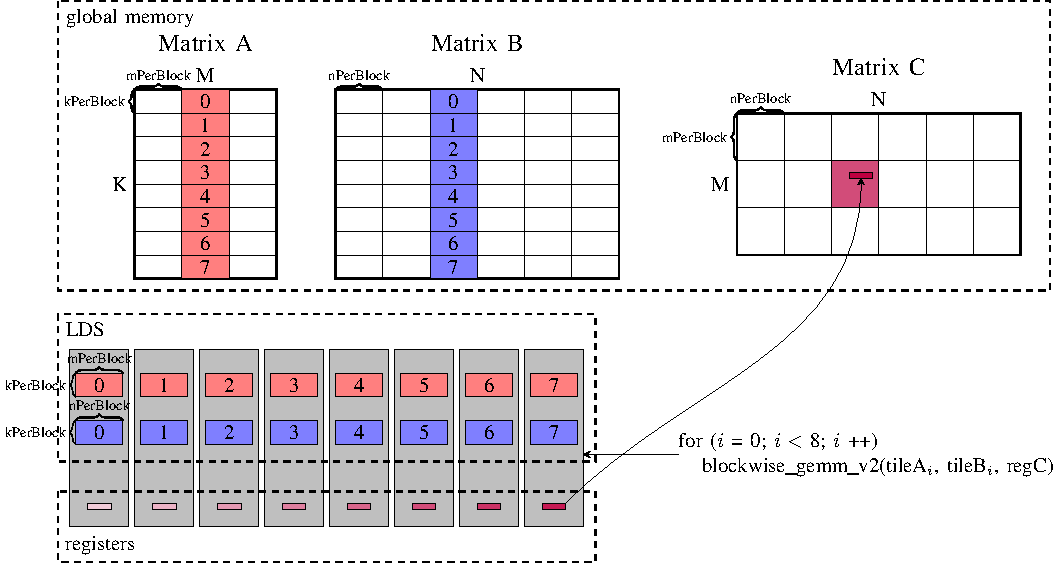
\includegraphics[width=5in]{gridwise_gemm_to_blockwise}
\end{frame}


\begin{frame}
  \frametitle{blockwise\_gemm to xdlops\_gemm}
  \vskip-2.5em
  %\centering
  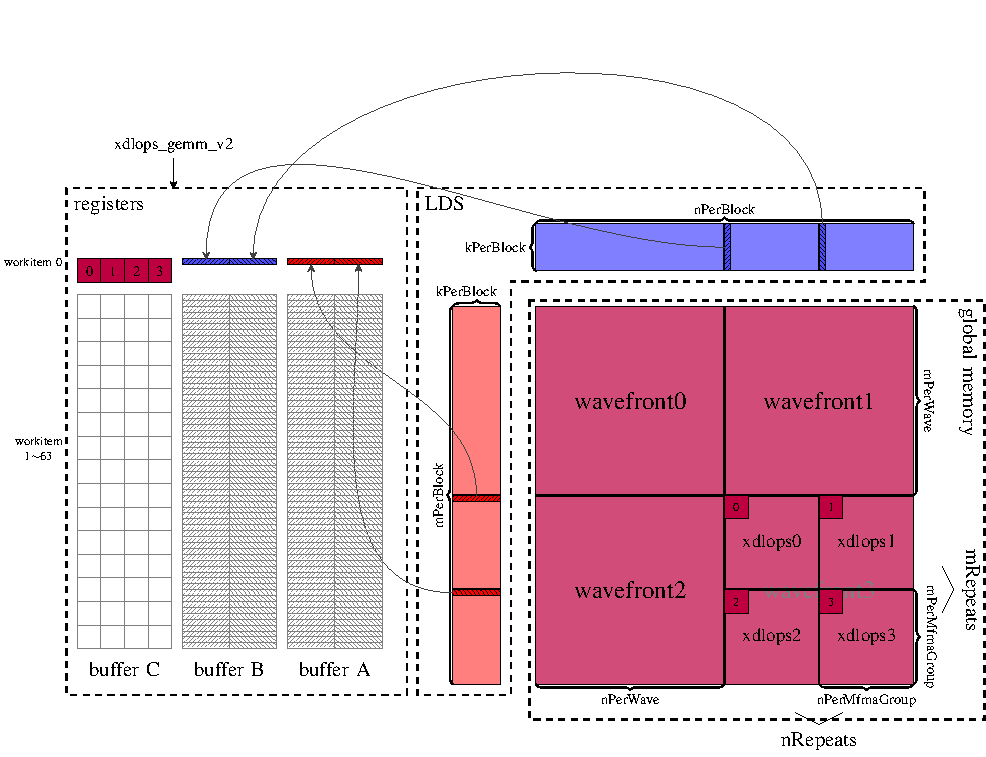
\includegraphics[width=4in]{blockwise_gemm_to_threadwise}
\end{frame}


\begin{frame}
  \frametitle{xdlops\_gemm to mfma instructions}

  \begin{tikzpicture}[overlay, remember picture]
    \coordinate (orig) at (0,.5);
    \draw [fill=cyan] (orig) circle (2pt);

    \node [below right, inner sep=0] at ($(orig)+(8, 1.2)$){
      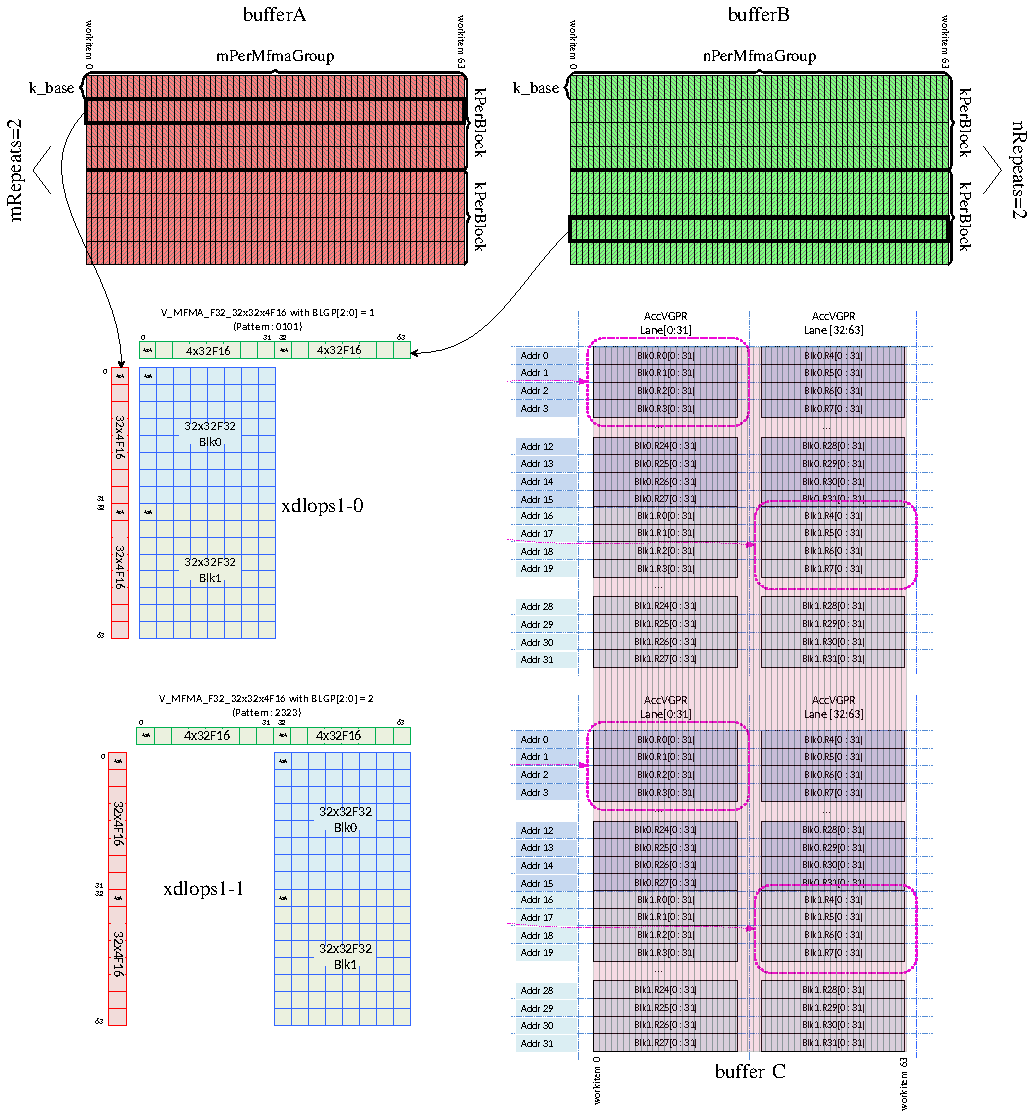
\includegraphics[width=3in]{threadwise_lowering}};

    \node [below right, align=left] at (orig) {
      - asdasf\\
      - adafad
    };
  \end{tikzpicture}


    %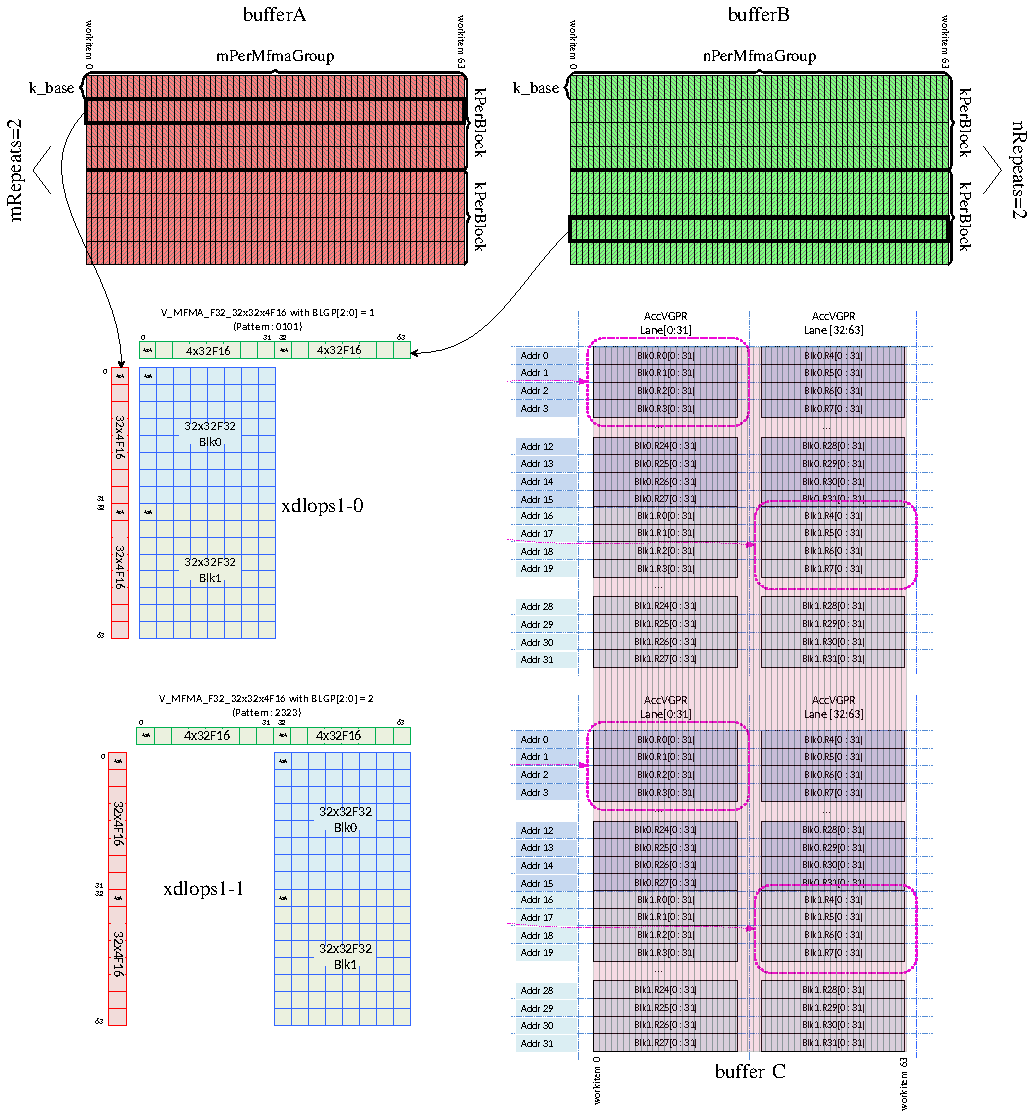
\includegraphics[width=3in]{threadwise_lowering}
  
\end{frame}



\section{}
	

	
\end{document}